\chapter{Independent set formulation of the partial row/column assignment problem} \label{chap:independent_set}

With the framework introduced in Section \ref{sec:hot_restart}, we basically translated the problem of the assignment of nonzeros to $A_r$ and $A_c$ (which is already another formulation of the matrix partitioning problem with the medium grain model) to the problem of an efficient computation of a permutation of the indices $0,\dots,m+n-1$. In this chapter, we will propose a method for this vector computation problem, which relies on concepts of the field of graph theory.

The main idea is somewhat similar to the principle that lead us to the development of the Separated Block Diagonal form of order 2 in Section \ref{sec:sbd2}. In that particular form of a partitioned matrix, as already argued, the blocks $\ddot{A}_{00}$ and $\ddot{A}_{44}$ are interesting, because they contain nonzeros with the property of being ``independent''. More precisely, those were rows and columns fully assigned to a processor and whose nonzeros didn't have any neighbor (a nonzero in the same row or column) which had a cut column/row. These nonzeros, then, could be assigned anywhere that they still did not cause communication.

The term \emph{independent}, in this reasoning, has to be defined very carefully: we want to look for a subset of $\{0,\dots,m+n-1\}$ which does not any communication, whenever we fully assign its rows to $A_r$ and its columns to $A_c$. With this definition, our goal is clear: we want to assign as much nonzeros as possible in this way, lowering consistently the upper bound on the communication volume that can be computed during the creation of $A_r$ and $A_c$.

To do so, we can employ a very well studied object in graph theory: the \textbf{independent set}. However, this requires a correct translation of our sparse matrix into a graph, in order to produce the desired result, which is described in Section \ref{sec:is_graph}. In Section \ref{sec:is_comp}, instead, we discuss the actual algorithm used to compute the maximum independent set in such graph.

\section{Graph construction} \label{sec:is_graph}

In order to retrieve the desired information from the graph, we need to construct it correctly from our sparse matrix. In our case, we can simply consider the graph whose adjacency matrix is none other than the sparsity pattern of our matrix $A$. This exact same formulation has already been studied for the matrix partitioning problem, under the name of \emph{bipartite graph model} by Hendrickson and Kolda \cite{hendrickson}, where the authors, after constructing the graph, discuss different algorithms for bipartite graph partitioning and come to the conclusion that the best strategy is using multilevel methods with Fiduccia-Mattheyses refinement.

More specifically, in this graph formulation we have that rows and columns are vertices, and we have the edge $(i,j)$ if $a_{ij} \neq 0$; the resulting graph is bipartite.

An example of such translation from matrix to graph is shown in Figure \ref{fig:bipartite_graph}, where we translate the matrix given in Figure \ref{fig:partition}. 

\begin{figure}[h]
	\centering
	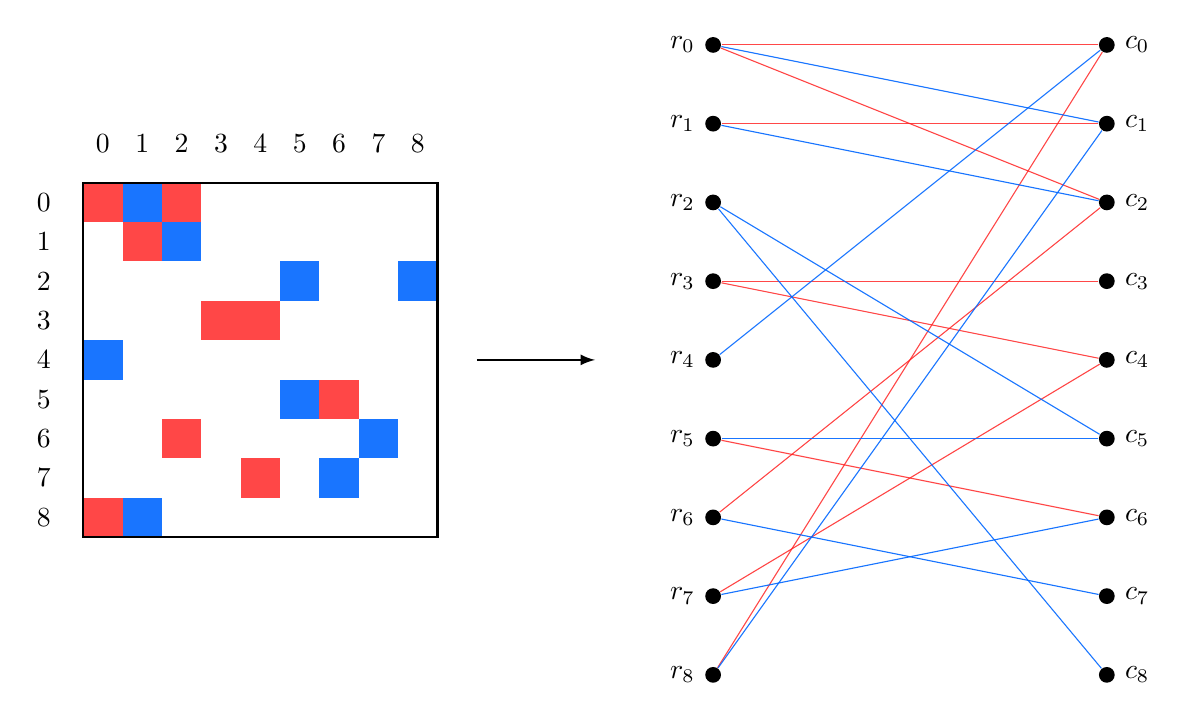
\begin{tikzpicture}[scale=0.5]
		\tikzstyle{myred}=[red!90,opacity=.8]
		\tikzstyle{myblue}=[blue!60!cyan,opacity=.9]
		\tikzstyle{mypurple}=[purple!80!blue,opacity=.9]
		\tikzstyle{myarrow}=[line width=1.3pt,>=latex,->]
		\tikzstyle{vertex} = [fill,shape=circle,node distance=100pt,minimum size=0.2cm,inner sep = 0pt]
		\foreach \x / \y in {1/1,1/3,2/2,4/5,4/4,7/3,8/5,6/7,9/1} { \fill[myred] ({\y-1},{-\x+1}) rectangle +(1,-1);}
		\foreach \x / \y in {1/2,2/3,3/6,3/9,6/6,5/1,7/8,8/7,9/2} { \fill[myblue] ({\y-1},{-\x+1}) rectangle +(1,-1);}
%		\draw[semithick] (0,-9) grid (9,0);
		\draw[thick] (0,-9) rectangle (9,0);

		\draw[myarrow,thick] (10,-4.5) -- (13,-4.5);

		\foreach \x in {0,...,8} { 
			\node[vertex,label=left:\(r_{\x}\)] (r\x) at (16,{3.5-2*\x}) {}; 
			\node[vertex,label=right:\(c_{\x}\)] (c\x) at (26,{3.5-2*\x}) {};
			\node at (-1,{-\x-0.5}) {\x};
			\node at (\x+0.5,1) {\x};
		}


			\foreach \x / \y in {0/0,0/2,1/1,3/4,3/3,6/2,7/4,5/6,8/0} { \draw[myred] (r\x) -- (c\y);}
			\foreach \x / \y in {0/1,1/2,2/5,2/8,5/5,4/0,6/7,7/6,8/1} { \draw[myblue] (r\x) -- (c\y);} 
		\end{tikzpicture}
		\caption{Graph constructed using the sparsity pattern of the matrix of Figure \ref{fig:partition} as adjacency matrix (rows and columns are vertices, nonzeros are edges). The edge color is the same of the corresponding nonzeros, but only to facilitate the understanding of this translation; in reality there is no distinction between edges. With $r_i$ we denote row $i$, whereas with $c_j$ we denote column $j$.} \label{fig:bipartite_graph}
	\end{figure}


\section{Computation of the independent set} \label{sec:is_comp}
\subsection{Hopcroft-Karp algorithm} \label{sec:hopcroft}

